Calcula el volumen de cada uno de los cuerpos geométricos que aparecen en la figura \ref{fig:vol_pris01}.

\begin{figure}[H]
    \centering
    \begin{subfigure}{.2\textwidth}
        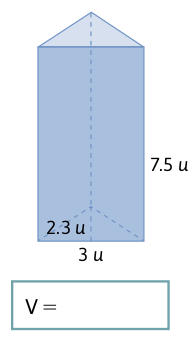
\includegraphics[width=\linewidth]{../images/20230319051022}
        \caption{Prisma triangular}
        \label{sfig:20230319051022}
    \end{subfigure}
    \begin{subfigure}{.25\textwidth}
        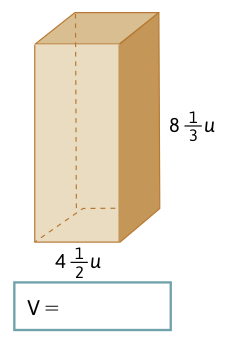
\includegraphics[width=\linewidth]{../images/20230319051030}
        \caption{Prisma cuadrangular}
        \label{sfig:20230319051030}
    \end{subfigure}
    \begin{subfigure}{.25\textwidth}
        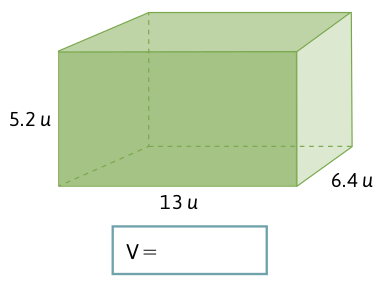
\includegraphics[width=\linewidth]{../images/20230319051039}
        \caption{Prisma rectangular}
        \label{sfig:20230319051039}
    \end{subfigure}
    \caption{Volúmenes de prismas rectos.}
    \label{fig:vol_pris01}
\end{figure}


